\documentclass{article}

\usepackage[paper=letterpaper,margin=2.5cm]{geometry} % Set Margins

%% Math and math fonts
\usepackage{ amsthm, amssymb, amsfonts}
\usepackage{bbm} % for \mathbbm{1}
\usepackage{amsmath}

% date
\usepackage[nodayofweek]{datetime}

% Color
\usepackage{color, xcolor}

% Misc
\usepackage{environ}  % \collect@body in asmmath
\usepackage{graphicx} % \includegraphics options
\usepackage{mdframed} % text boxes
\usepackage{indentfirst} % Indent first paragraph after section header
\usepackage[shortlabels]{enumitem} % Control enumerate items with [(a)]
\usepackage{comment} % Comments
\usepackage{fancyhdr} % Headers and footers

% Tables
\usepackage{array}

% Sub-figures and figure placement
\usepackage{caption}
\usepackage{subcaption}
\usepackage{float} 

% Graphing
\usepackage{pgfplots}
\pgfplotsset{compat=1.17}
\usepackage{tikz}

% Title Placement
\usepackage{titling}
\setlength{\droptitle}{-6em}

%set indent to 
\setlength{\parindent}{0pt}

% Hyper refs
\usepackage{hyperref}
\hypersetup{
    colorlinks=true,
    linkcolor=blue,
    urlcolor  = blue,
    filecolor=magenta,      
    urlcolor=blue,
    citecolor = blue,
    anchorcolor = blue
}

% % Citation management
\usepackage{natbib}
\bibliographystyle{abbrvnat}
\setcitestyle{authordate,open={(},close={)}}

\pagestyle{fancy}

\usepackage[paper=letterpaper,margin=2.5cm]{geometry} % Set Margins

%% Math and math fonts
\usepackage{amsmath, amsthm, amssymb, amsfonts}
\usepackage{bbm} % for \mathbbm{1}

% date
\usepackage[nodayofweek]{datetime}

% Color
\usepackage{color, xcolor}

% Misc
\usepackage{environ}  % \collect@body in asmmath
\usepackage{graphicx} % \includegraphics options
\usepackage{mdframed} % text boxes
\usepackage{indentfirst} % Indent first paragraph after section header
\usepackage{comment} % Comments
\usepackage{fancyhdr} % Headers and footers

% Tables
\usepackage{array}

% Sub-figures and figure placement
\usepackage{caption}
% \usepackage{subcaption}
\usepackage{float} 

% Graphing
\usepackage{pgfplots}
\pgfplotsset{compat=1.17}
\usepackage{tikz}

% Title Placement
\usepackage{titling}
\setlength{\droptitle}{-6em}

%set indent to 
\setlength{\parindent}{0pt}

% Hyper refs
\usepackage{hyperref}
\hypersetup{
    colorlinks=true,
    linkcolor=blue,
    urlcolor  = blue,
    filecolor=magenta,      
    urlcolor=blue,
    citecolor = blue,
    anchorcolor = blue
}

% % Citation management
\usepackage{natbib}
\bibliographystyle{abbrvnat}
\setcitestyle{authordate,open={(},close={)}}

\newcolumntype{M}{>{$}c<{$}} % Define a new column type for math mode


% ----------------------------------------
% TITLE
% ----------------------------------------

\pagestyle{fancy}

\lhead{Creel}
\chead{Review}
\rhead{AMES}

\title{AMES Midterm Review}
\author{Andie Creel}

\begin{document}
\maketitle

\section{Exponential functions}
What does an exponential function really mean? 
\begin{align}
    f(x) = e^x\\
    f'(x) = e^x
\end{align}
$f(x)$ is a function where the \textbf{slope} of the function increases \textbf{by the rate that f(x)} is increasing. That is why the derivative of $e^x$ is still $e^x$. 

\section{Percent Change}
Let's say you have a function that models an outcome of interest, 
\begin{align}
    y = f(x)
\end{align}

Consider the case where you are interested in the percent change of that outcome (\textit{i.e.} \% change in $y$) rather than the level of the outcome (\textit{i.e.} $y$ itself). \\

What is a transformation of the function that would give us a percent change in y? Taking the derivative of the log of the function. 
\begin{align}
    g(x) &= ln(f(x))\\
    \text{\% change in y} &= g'(x)\\
    &= \frac{d}{dx}  ln(f(x))\\
    &= \frac{1}{f(x)} f'(x) \\
    & = \frac{f'(x)}{f(x)} \label{perc_change}\\
    &= \frac{\Delta f(x)}{f(x)}
\end{align}
where we've used the properties of logs and the change rule. \\

\textbf{Note: Log to percent change interpretations apply to more than just $f(x)$} \\
Any time you see a function that describes a variable in the form of \ref{perc_change}, you can interpret it as a percent change of the variable. For example, let's say you are interested in a variable that is the slope of a function, $z = f'(x)$.  You want to write down the \textit{percent change of $z$, or the percent change in the slope of $f(x)$}. You can write that as, 
\begin{align}	
	\text{\% change in z} = \frac{f'(x)}{f''(x)}
\end{align}

You could simplify this expression by using a log 
\begin{align}	
	\text{\% change in z} &= ln(f'(x)) \label{eleven}\\
	&=  \frac{f'(x)}{f''(x)} \label{twelve}
\end{align}

because \ref{twelve} follows from \ref{eleven} after using log rules and the chain rule. 

\section{Draw graphs when you know what they are}

\begin{figure}[htp]
    \centering
        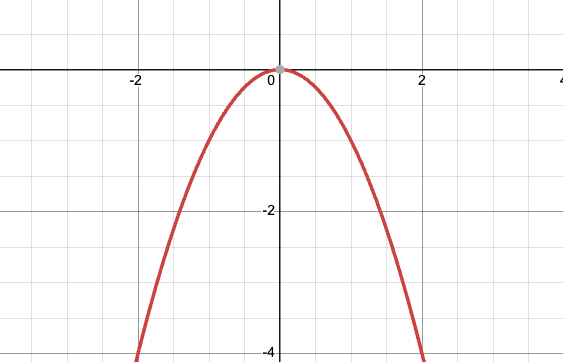
\includegraphics[width=0.35\textwidth]{Screen Shot 2023-10-23 at 4.53.45 PM.png}
    \caption{$-x^2$}
    % \label{fig:sample}
\end{figure}

If you think you can draw a graph with the information you have, sketch it out. This will give you intuition. \\

Let's say I have the function $y = f(x) = -x^2$\\ 

What's the sign of the derivative when x is less than 0? (positive) \\

What's the sign of the derivative when x if greater than zero? (negative) \\

What's the sign if the derivative when $x = 0$? (zero)\\

All these questions are not-tedious to answer when looking at a graph, but harder without. 

\section{Finding max and min with first and second derivative}

Consider the function $f(x)$. \\

What level of $x$ maximizes or minimizes $f(x)$? We want to know when the slope is zero (at the top of the "mound"). Therefore, to find the max or min, take the first derivative and set it equal to zero. Solve that equation for $x$, which will be the level of $x$ that maximizes $f(x)$. \\

How do we know if it's a max or min? Take the second derivative and plug in that value of x. If it's negative, then it's a maximum (frowny face). This is also a concave function (looks like a cave). If it's positive, then it's a minimum (smiley face). This is also a convex function (kind of looks like a v). 


\section{Convex Function vs Convex Set}
A convex function and a convex set are two completely different concepts that use the same world. They are not related. A convex function is a function whose second derivative is positive. A convex set is a set where you can draw a line between any points in the set, and all other points the connecting line passes through are also in the set. For example, a circle is a convex set. A star is not a convex set. 
 

\section{Taylor Series}

We know that straight lines are good approximates because a line is a conditional mean, and means are good at minimizing error.\\

Series are good approximators of sequences of numbers because series are functions. \\

A \textbf{Taylor Series} is an extremely useful series for approximating the relationship of a sequence of numbers (data is a sequence of numbers). Taylor series underpins a lot of the math we do today, particularly for any relationship that isn't linear. 

\begin{align}
    f(x) = f(a) + \frac{f'(a)}{1!}(x-a)^1 + \frac{f''(a)}{2!}(x-a)^2 + \frac{f'''(a)}{3!}(x-a)^3 + ... + \frac{f^k(a)}{k!}(x-a)^k + R
\end{align}
where $R$ is the residual.\\


\subsection{0th order Taylor Series}
Consider a 0th order taylor series: it would be a mean aka just a flat line equal to $f(a)$. \\

If you're only looking at the means of a dataset, that means you're doing a 0th order taylor approximation.

\subsection{First order Taylor Series}

Consider a first order taylor series: 
\begin{align}
    f(x) &= f(a) + \frac{f'(a)}{1!}(x-a)^1 \\
    &= A + B (x-a) \\
    &= A -aB + Bx\\
    &= m + Bx
\end{align}
It's a line with a slope. A first order Taylor series is a linear approximation. Linear regression is a first order Taylor approximation. \\

\subsection{Discussion of models}
Any Taylor Series approximation is a model. If someone says "I don't do models, let's only do means" they actually \textit{are} suggesting a model. A mean is a model, it's a zero order Taylor Series approximation! 

Higher order Taylor Series will approximate an underlying function better than a lower order. \textit{However,} we do not always have enough data to fit a higher order Taylor series because it would require more estimating parameters and your data set may not have enough power (aka enough data) to do so. \\

More on Taylor series: \url{https://github.com/a5creel/AMES/blob/main/class_notes/5_weds/main.pdf}. 


\section{Derivative and Integral Rules}

\begin{tabular}{|M|M|M|c|}
  \hline
  \text{Function} & \text{Derivative}  & \text{Anti-Derivative} & Name\\
    \hline
      F(x) & F'(x) & \int F'(x) dx  & \\
      \hline
      x & \frac{dx}{dx} = 1 \rightarrow dx = 1 dx & \int dx = x + c & wrt variable\\
      \hline
      \alpha x & \alpha \frac{dx}{dx} = \alpha \rightarrow \alpha dx & \int \alpha dx = \alpha \int dx = \alpha x + c & constant\\
      \hline
      x^N & \frac{dF}{dx} = Nx^{N-1} \rightarrow dF = Nx^{N-1} dx & \int N x^{N-1}dx = \frac{1}{N}x^N +c & power rule\\
      \hline
      g(x) + h(x) & \frac{d g(x)}{dx} + \frac{dh(x)}{dx}  \rightarrow dF = (g'(x) + h'(x)) dx & \int (g'(x) + h'(x)) dx = \int g'(x) dx + \int h'(x) dx & linear operator \\
      \hline 
      e^x & \frac{dF}{dx} = e^x \rightarrow dF = e^x dx & \int e^x dx = e^x + c & exponentials\\
      \hline
      ln(x)  & \frac{d ln(x)}{dx} = \frac{1}{x} \rightarrow dF = \frac{1}{x} dx & \int \frac{1}{x} dx = \int \frac{dx}{x} = \int x^{-1}dx = ln(x) + c & logs\\
      \hline 
     f(x) =  g(h(x)) & \frac{df}{dx} = \frac{dg}{dh}\frac{dh}{dx} & \int g(h(x)) dx & chain rule/ \\
      & & u = h(x), \frac{du}{dx} = h'(x) \implies dx = \frac{du}{h'(x)} & u-substitution \\
      & & \int g(u) \frac{du}{h'(x)} & \\
      \hline
      ln(F(x)) & \frac{dF}{dx} = \frac{1}{F(x)} F'(x) =\frac{F'(x)}{F(X)} & \text{do a u-sub}& percent change\\
      \hline
      g(x) h(x) & g'(x) h(x) + g(x) h'(x) & \text{integration by parts}  & product rule \\
      \hline
      g(x)^{-1}h(x) & \frac{h'(x) g(x_ - g'(x) h(x)}{g(x)^2} & \text{integration by parts} & quotient rule \\
      \hline
      
\end{tabular}

\section{Implicit function theorem}
Consider 
\begin{align}
    F(x,y) \\
    d F = F_x dx + F_y dy \\ 
\end{align}
where 
\begin{align}
    F_x = \frac{\partial F}{\partial x} \\
    F_y = \frac{\partial F}{\partial y}
\end{align}

When you're at an equilibrium, $F$ will not be changing 
\begin{align}
    0 = F_x dx + F_y dy \implies \\
    - \frac{F_x}{F_y} = \frac{dy}{dx}
\end{align}
\textbf{Interpretation}: When at an equilibrium, the change in $y$ w.r.t $x$ will equal the negative ratio of the partial derivatives.  





\section{pset 1 Q 1}
Function: 
\begin{align}
    f(x) &= x^2 ln(x^2)\\
\end{align}
first derivative: 
\begin{align}
    f'(x) &= 2x ln(x^2) + x^2 \frac{1}{x^2}2x\\
    &= 2x ln(x^2) + 2x \\
\end{align}
second derivative
\begin{align}
    f''(x) &= 2ln(x^2) + 2x \frac{1}{x^2} 2x + 2\\
    &= 2ln(x^2) + 6
\end{align}

To find point of inflection, set second derivative to 0 and solve for x
\begin{align}
    2ln(x^2) + 6 = 0\\
    ln(x^2) = -3 \\
    x^2 = exp(-3) \\
    x = exp(-3)^{1/2}
\end{align}

I think there is a typo for the inflection point in the answer key. 

\section{integration by parts }
section 4 \url{https://github.com/a5creel/AMES/blob/main/class_notes/6_weds/main.pdf}

\end{document}